
\section{\textbf{Procedimentos Metodológicos}}\label{cap:metodologia}
    
    \subsection{Ajuste e interpolação por isócronas}\label{sec:isocfit}
    Isócronas são úteis para estimar a massa de uma estrela com base no diagrama HR (DHR), assumindo que a perda de massa é desprezível. Usamos modelos teóricos de isócronas de \citeonline{siess2000internet} e \citeonline{baraffe2015new}, com massas entre \(0.1 ~M_\odot\leq M \leq 1.4~M_\odot\). O ajuste das isócronas foi feito com uma abordagem similar à regressão de N-Vizinhos, prevendo a massa pela interpolação das isócronas mais próximas.
    
    
    \begin{figure}[!h]
    	\centering
    	\caption[Exemplo de análise visual do método de ajuste de isócronas.] {Exemplo de visualização para diagnosticar os resultados obtidos mediante o método de ajuste de isócronas. No gráfico está o DHR para uma estrela do ONC.}
    	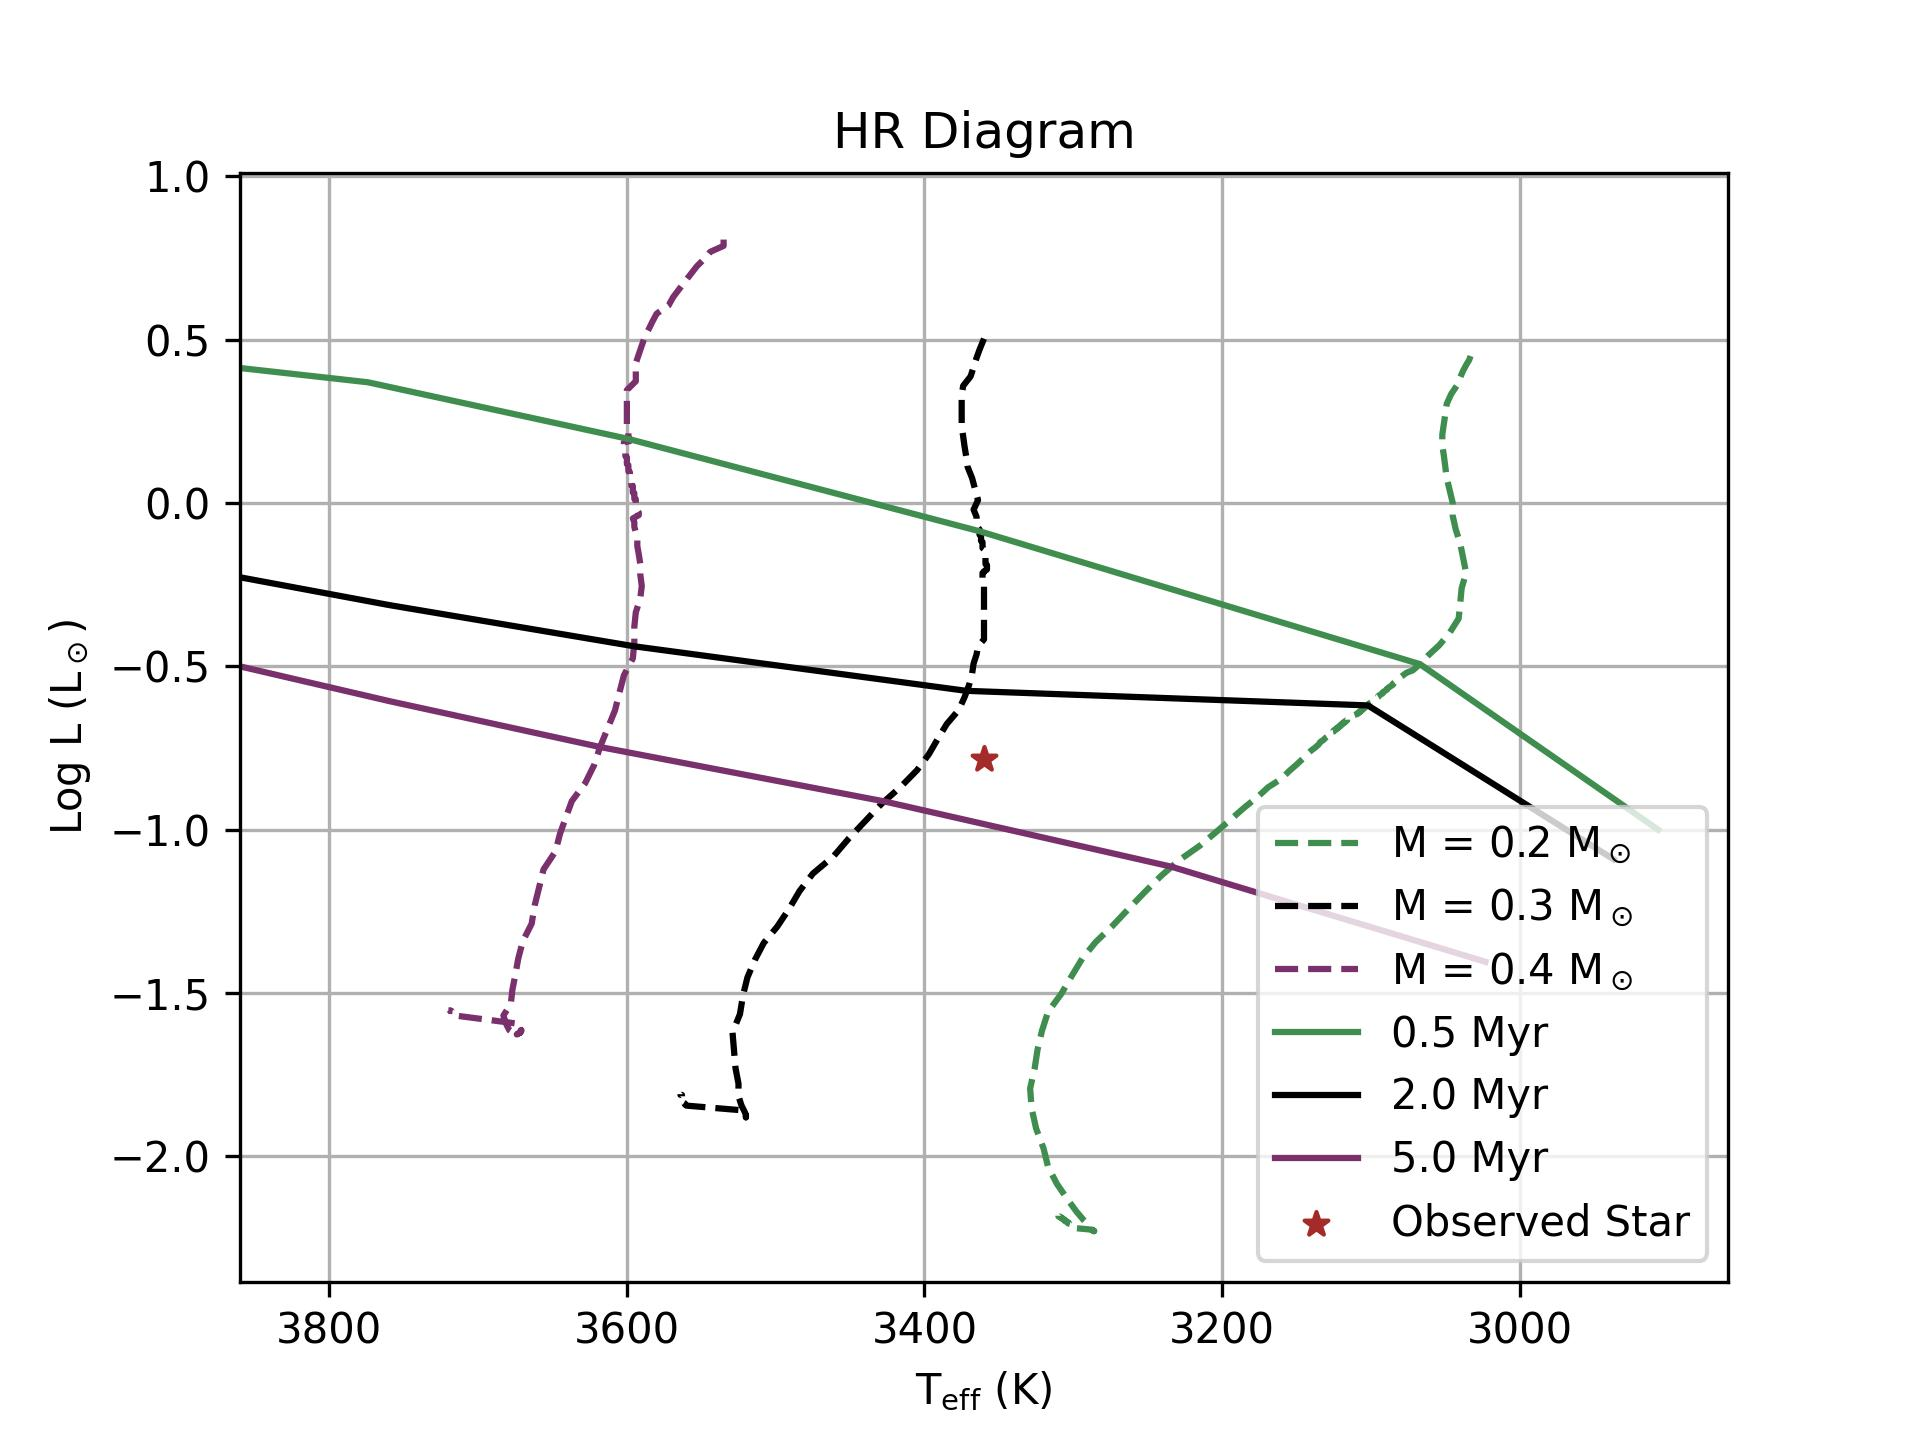
\includegraphics[width=0.75\linewidth]{./04-figuras/hrd_star.jpg}
    	\label{fig:hrd_isocfit}
    \end{figure}
    
     Para estimar a massa e a idade inicial, o código compara a temperatura efetiva (\(T_{ef}\)) e a luminosidade (\textit{L}) do objeto com as trilhas evolutivas e isócronas, minimizando a equação (\ref{eq:delta}).
     
    \begin{equation}\label{eq:delta}
    	\delta = \sqrt{\left(T_{\text{ef}}-T_{\text{ef},\,0}\right)^2 + (L - L_0)^2} ~,
    \end{equation}
    
    onde \(T_{\text{ef},\,0}\) e \(L_0\) são extraídas das trilhas, enquanto \(T_{\text{ef}}\) e \(L\) são valores calculados ou retirados dos catálogos utilizados. O ajuste é visualizado no DHR, como mostrado na Figura \ref{fig:hrd_isocfit}. O código oferece uma estimativa de massa refinada pela interpolação das isócronas vizinhas.
    Erros nas estimativas de extinção ou temperatura efetiva podem introduzir erros sistemáticos nas idades e massas inferidas, impactando as escalas de tempo associadas à dissipação do disco protoplanetário e à formação planetária.
    
    \subsection{Massa Estelar}\label{sec:massa_estelar}
    A massa individual de uma estrela não-binária pode ser calculada a partir de uma lei de potência como descrita nas equações (\ref{eq:massai}) e (\ref{eq:massa1}), onde o coeficiente \(\alpha\) varia com estágio evolutivo da estrela e \(\beta\) é uma constante de proporcionalidade.
    
    \begin{equation}
    	\label{eq:massai}
    	M^* =  \beta L^\alpha
    \end{equation}
    
    \begin{equation}
    	\label{eq:massa1}
    	\log(M^*) =  \alpha L + \log(\beta)
    \end{equation}
    
    Podemos descrever a luminosidade a partir da sua magnitude absoluta (\(\Lambda\)) e assim, evitar a necessidade dos dados necessários para calculá-la, modelando então uma relação do tipo (\ref{eq:massa2}):
    
    \begin{equation}
    	\label{eq:massa2}
    	\log(M^*) =  \gamma \, \Lambda + \eta ~,
    \end{equation}
	onde \(\gamma\) e \(\eta\) são os coeficientes para a relação massa-magnitude.
    
    O objetivo é desenvolver um procedimento automatizado para modelar uma relação entre massa e magnitude de estrelas em aglomerados estelares, com foco em objetos mais jovens e assim obter a massa individual das mesmas. Dada a falta de um conjunto de calibração de estrelas de referência não-enviesado que compartilhem as mesmas características, como um conjunto de estrelas binárias, recorremos a bibliotecas sintéticas de modelos teóricos de isócronas.
    
    Todos os cálculos para determinação da massa e a análise estatística realizada sobre os modelos de regressão foram realizados a partir de um programa próprio\footnote{ \url{https://github.com/Gomes-JP/stelar}}, escrito em \textit{Python}, a fim de automatizar as tarefas para todos os aglomerados.  
    
    \subsection{Aprendizagem de Máquina}
    A metodologia aplicada para a relação massa-magnitude utiliza técnicas de aprendizagem de máquina (\textit{machine learning}) para estimar a massa de estrelas jovens em aglomerados estelares. A partir dos dados teóricos de isócronas, são construídos modelos de regressão, aproveitando a flexibilidade do aprendizado de máquina para lidar com possíveis não linearidades que os métodos tradicionais poderiam ignorar. A combinação de diversos algoritmos visa melhorar a precisão das estimativas de massa.
    
    A técnica de re-amostragem \textit{k-fold} foi usada, dividindo os dados em 10 conjuntos. Nove conjuntos foram usados para treinar o modelo e um para validação, repetindo o processo 10 vezes para garantir que os modelos não estivessem se ajustando muito bem ao conjunto de dados anteriormente observado, mas ineficaz para prever novos resultados. A otimização dos hiper parâmetros\footnote{ Um parâmetro que define qualquer parte configurável do processo de aprendizagem de um modelo e não um parâmetro do modelo em si.} foi realizada por meio de uma busca em grade (\textit{grid search}), minimizando o erro quadrático médio negativo (NMSE), ajustando cada modelo com o melhor conjunto de parâmetros.
    
    As técnicas de regressão de aprendizado de máquina visam ajustar modelos que minimizem a raiz do resíduo quadrático médio (RMSE), dado pela Equação(\ref{sr}).
    
    \begin{equation}
    	\label{sr}
    	RMSE = \sqrt{\frac{1}{k}\sum_{j=0}^{k} [f(x_j) - y_j]^2}
    \end{equation}
    
    Aqui, \( f \) representa a função de regressão que estima \( y_j \) a partir dos dados de entrada \( x_j \). A escolha de \( f \) varia entre os diferentes métodos de regressão disponíveis na biblioteca \textbf{Scikit-Learn} listados abaixo:
    
    \begin{itemize}
    	\item[(i)] \textbf{Regressão Linear}
    	
    	\item[(ii)] \textbf{Regressão Bayesiana}
    	
    	\item[(iii)] \textbf{Regressão de Vetores de Suporte (Support Vector Regressor, SVR)}
    	\item[(iv)] \textbf{Árvore de Decisão (Decision Tree)}
    	
    	\item[(v)] \textbf{Floresta Aleatória (Random Forest)}
    	
    	\item[(vi)] \textbf{Impulsionamento em Gradiente}
    	
    	\item[(vii)] \textbf{Impulsionamento Ada}
    	
    	\item[(viii)] \textbf{K-ésimos Vizinhos mais Próximos (KNN)}
    	
    	\item[(ix)] \textbf{Rede Elástica (ElasticNet)}
    \end{itemize}       
    
    
    \subsection{Ferramentas estatísticas e análise dos resultados}\label{sec:estatistica}
    A probabilidade e a estatística são importantes quando há falta de informações completas sobre as condições iniciais de um sistema.
    
    Para avaliar a qualidade dos modelos de determinação de massa, usamos métricas como RMSE (erro quadrático médio), MAE (erro absoluto médio), coeficiente de determinação (\(R^2\)) e o Critério de Informação de Akaike (AIC). Dividimos os dados teóricos dos modelos de isócronas em duas partes: uma para treinar os modelos e outra para validar sua qualidade.
    
    Também realizamos uma análise comparativa utilizando regressão linear por mínimos quadrados ordinários (OLS) com a biblioteca \textit{Statsmodels} para comparar os dados de treino e teste. Para automatizar a seleção do melhor modelo, criamos uma nova métrica de pontuação, onde as métricas são normalizadas e ponderadas, considerando que \(R^2\) é inverso aos demais e o AIC pode ser negativo.
    
    A matriz das métricas (\(\mathcal{M}\)) e a matriz de pesos (\(\mathcal{P}\)) foram definidas, considerando a frequência de uso na literatura. O AIC, por refletir a verossimilhança do modelo com as isócronas teóricas, recebeu o menor peso.
    
    \begin{equation}
    	\label{matrix:metric}
    	\mathcal{M}=\begin{bmatrix}
    		{RMSE}_{1} & {MAE}_{1} & (1 - {R^2}_{1}) & {AIC}_{1} \\
    		{RMSE}_{2} & {MAE}_{2} & (1 - {R^2}_{2}) & {AIC}_{2} \\
    		\vdots & \vdots & \vdots & \vdots \\
    		{RMSE}_{n} & {MAE}_{n} & (1 - {R^2}_{n}) & {AIC}_{n}
    	\end{bmatrix}
    \end{equation}
    
    \begin{equation}
    	\label{matrix:pesos}
    	\mathcal{P}=\begin{bmatrix}
    		0.35 & 0.25 & 0.30 & 0.10  
    	\end{bmatrix}
    \end{equation}
    
    Para selecionar o melhor modelo, calculamos a matriz das pontuações (\(\mathcal{{S}}\)) utilizando a fórmula:
    
    \begin{equation}
    	\label{eq:score}
    	\mathcal{S} = \mathcal{\hat{M}} \cdot \mathcal{P}^T
    \end{equation}
    onde \(\mathcal{\hat{M}}\) é a matriz normalizada das métricas seguindo a relação da equação (\ref{eq:norm}). 
    
    \begin{equation}
    	\label{eq:norm}
    	\hat{x} = \frac{x - x_{min}} {x_{max} - x_{min}}
    \end{equation}
    
    A menor pontuação (\textit{s}) da matriz \(\mathcal{{S}}\) indica o melhor modelo. Nos casos de possíveis degenerescências nos resultados, foi adotado o modelo mais simples. Assim realizando novamente o treinamento utilizando a amostra total dos dados.
    
    Essa abordagem permite uma comparação direta entre modelos, considerando um conjunto de métricas relevantes. Para verificar a adequação do melhor modelo gerado para o aglomerado estudado, utilizaremos os seguintes conceitos estatísticos]:
    
    \begin{itemize}
    	\item[(i)] \textbf{Correlação}
    	\item[(ii)] \textbf{Normalidade dos Resíduos}
    	\item[(iii)] \textbf{Cedasticidade}
    	\item[(iv)] \textbf{\textit{Outliers} e influência}
    \end{itemize}
    
    Na análise comparativa, o coeficiente \(R^2\) é fundamental para avaliar a qualidade do ajuste do modelo aos dados. Um valor de \(R^2 \geq 0.75\) foi considerado indicativo de forte correlação neste estudo.
    
    Para verificar se os erros são aleatórios ou indicam algum viés, aplicamos o teste de normalidade de Jarque-Bera, adequado para amostras grandes (\(n \geq 500\)). A hipótese nula assume que os dados seguem uma distribuição normal. Caso o p-valor seja inferior ao nível de significância adotado (\(\alpha = 0.05\)), rejeitamos a hipótese de normalidade, indicando possíveis desvios sistemáticos.